\section*{Лабораторная работа}
\textbf{Содержание проекта:} Команда разработчиков из \textbf{16 человек} занимается созданием карты города на основе собственного модуля отображения. Проект должен быть завершен в течение \textbf{6 месяцев}. Бюджет проекта: 50 000 рублей.

\subsection*{Задание №1: Выравнивание загрузки ресурсов в проекте}

В задании №1 нужно было ликвидировать перегрузку ресурсов в проекте (рис. \ref{p1}).
\begin{figure}[!h]
	\centering
	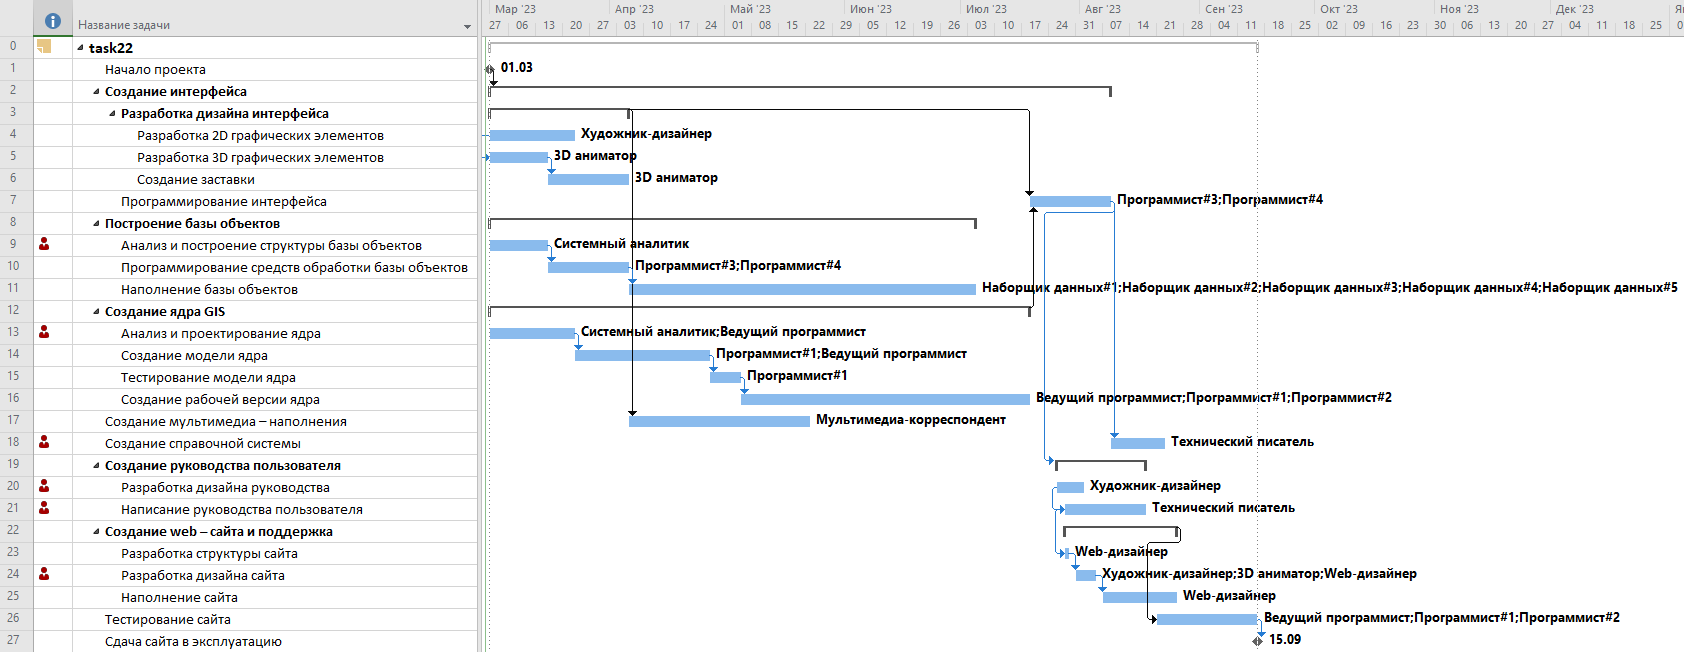
\includegraphics[width=1\linewidth]{inc/img/1.png}
	\caption{Перегрузка ресурсов в проекте}
	\label{p1}
\end{figure}

По диаграмме Ганта видно, что некоторые ресурсы используются для нескольких задач одновременно, что решается переносом соответствующих задач на допустимую дату. На рисунке \ref{p2} изображена исправленная диаграмма Ганта.

\begin{figure}[!h]
	\centering
	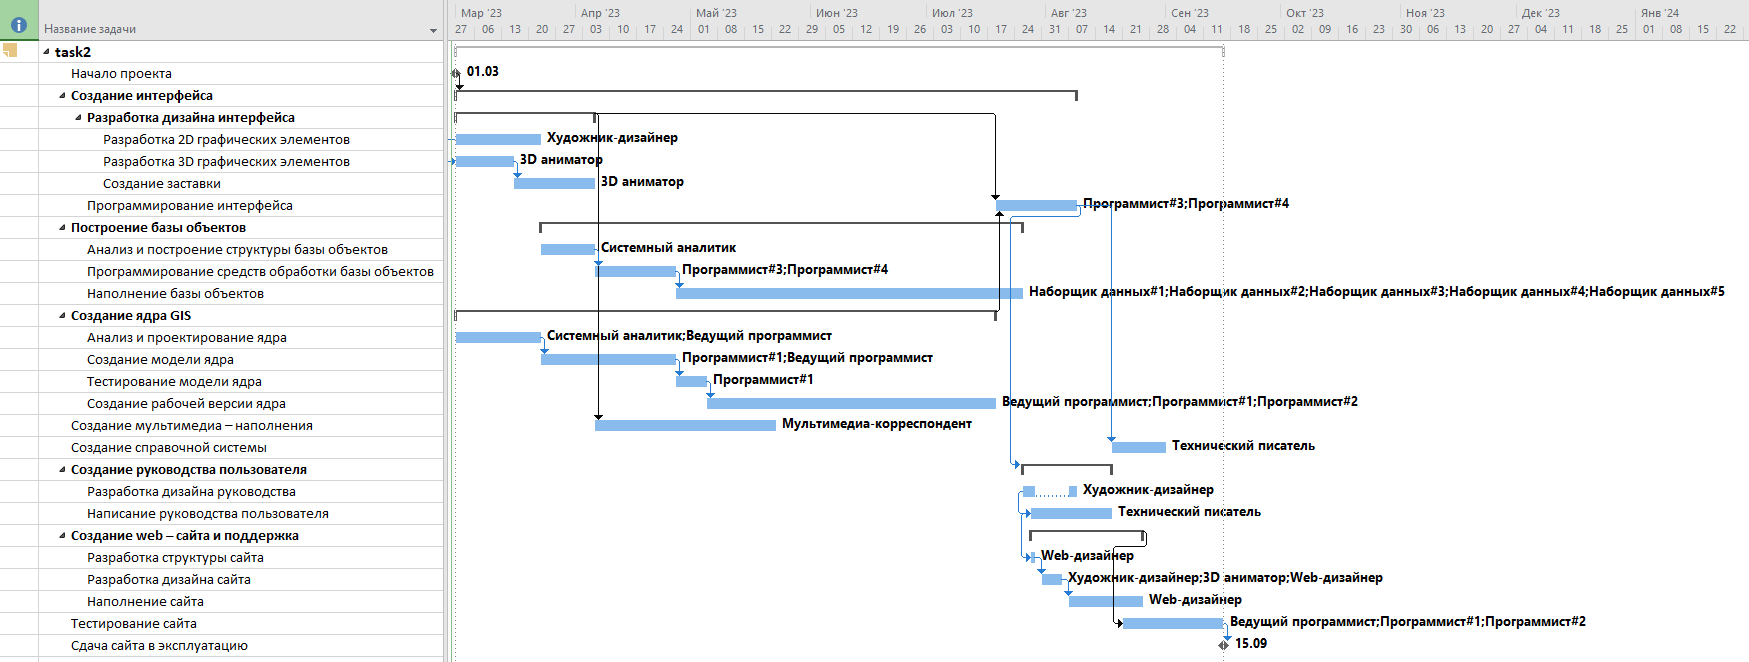
\includegraphics[width=1\linewidth]{inc/img/2.png}
	\caption{Исправленная диаграмма Ганта}
	\label{p2}
\end{figure}

\newpage
\subsection*{Задание №2: Учет периодических задач в плане проекта}

При добавление еженедельных совещаний по средам, ресурсы снова стали перегруженными (рис. \ref{p3})

\begin{figure}[!h]
	\centering
	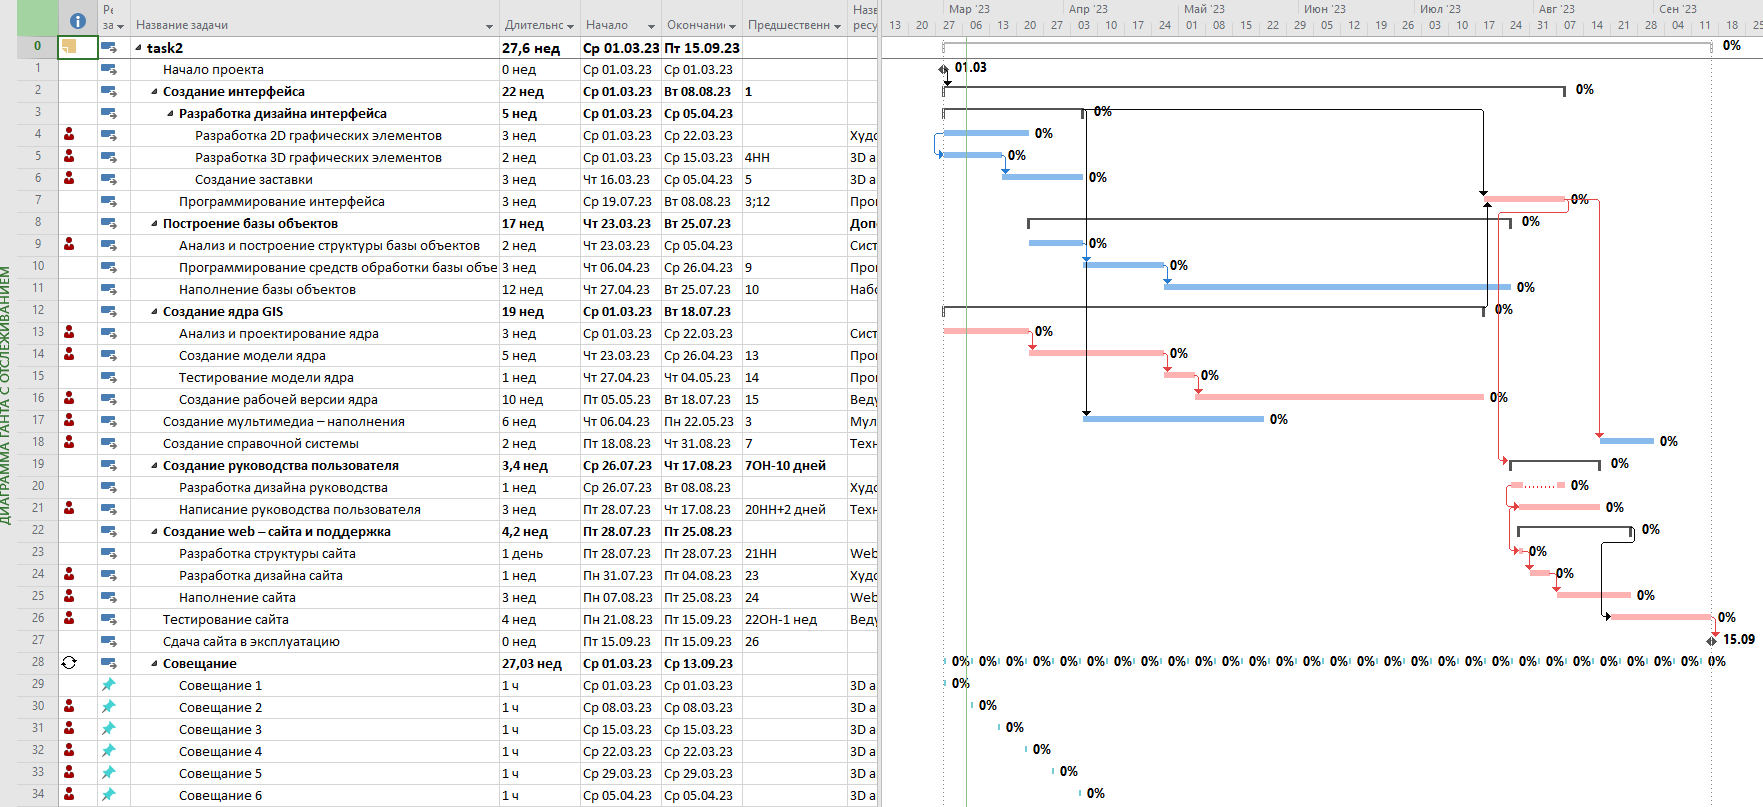
\includegraphics[width=1\linewidth]{inc/img/3.png}
	\caption{Перегрузка ресурсов после добавления совещаний}
	\label{p3}
\end{figure}

Большое количество перегрузок было устранено с помощью выравнивания (рис. \ref{p4})

\begin{figure}[!h]
	\centering
	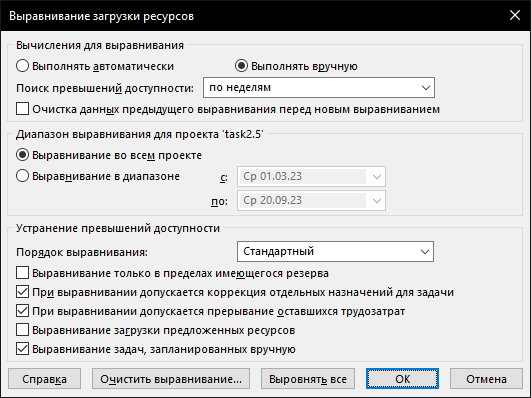
\includegraphics[width=0.8\linewidth]{inc/img/4.png}
	\caption{Настройки выравнивания}
	\label{p4}
\end{figure}
\newpage
После избавления от перегрузок ресурсов, выполнения проекта увеличилось на 5 дней (рис. \ref{p5})

\begin{figure}[!h]
	\centering
	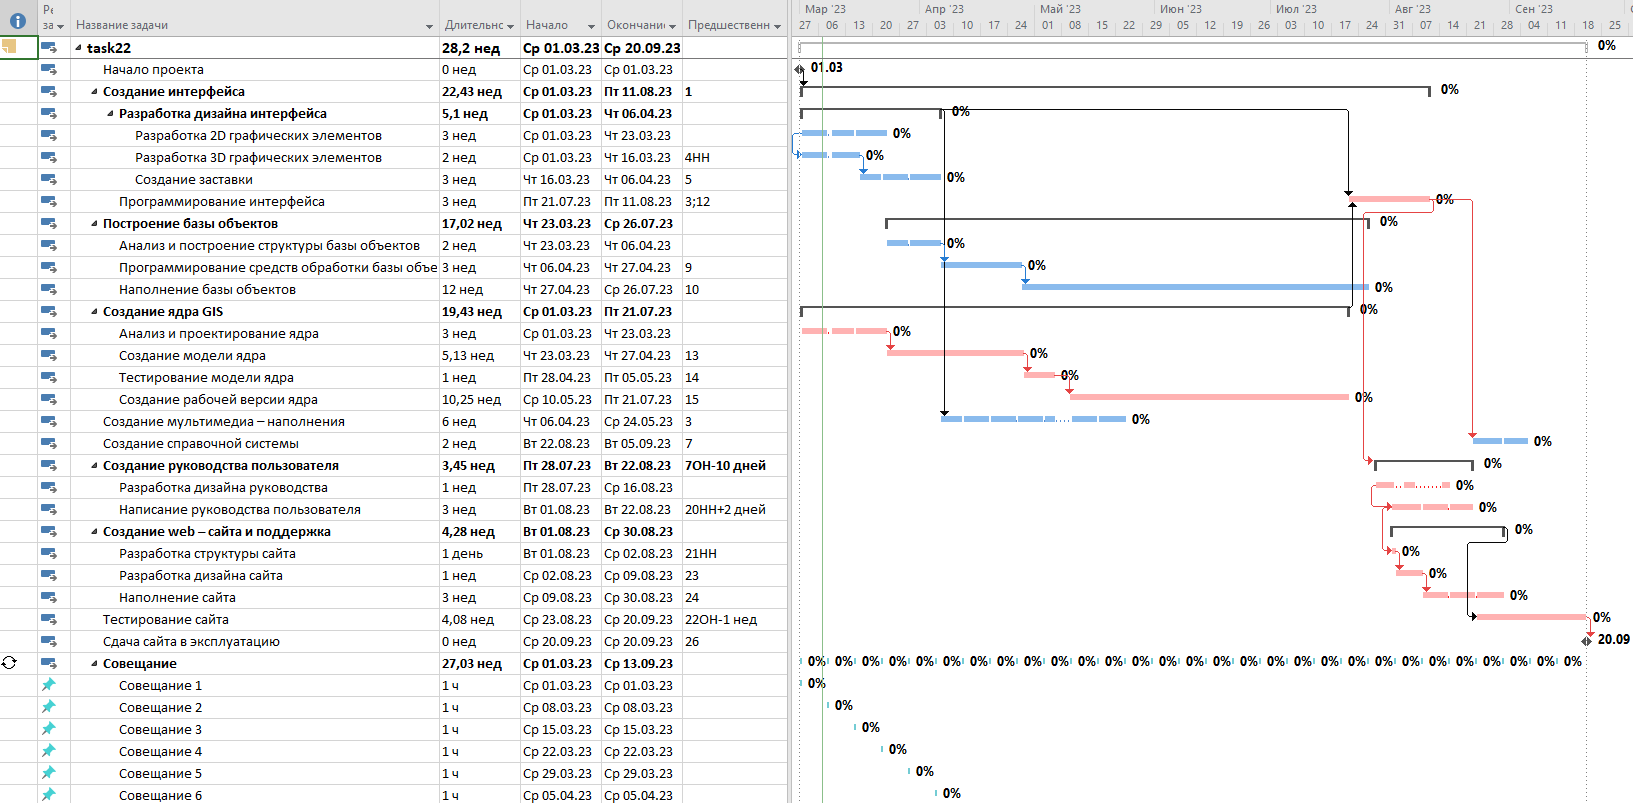
\includegraphics[width=1\linewidth]{inc/img/5.png}
	\caption{Диаграмма Ганта после выравнивания}
	\label{p5}
\end{figure}
\newpage
Кроме этого, поскольку в совещаниях участвует большинство ресурсов, затраты на них очень большие (рис. \ref{p6}), в следствии чего превышается бюджет всего проекта.

\begin{figure}[!h]
	\centering
	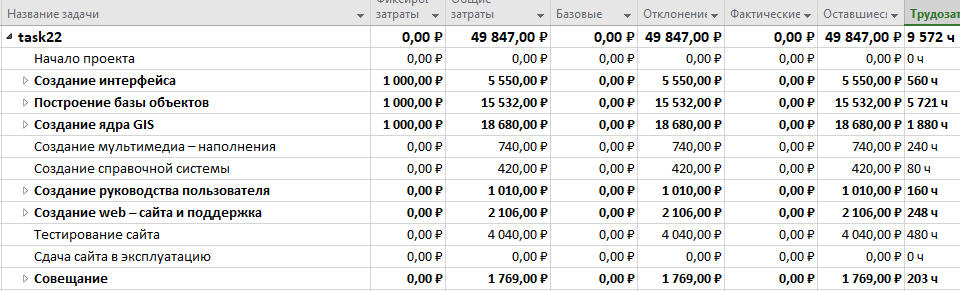
\includegraphics[width=1\linewidth]{inc/img/6.png}
	\caption{Затраты на совещания}
	\label{p6}
\end{figure}

\subsection*{Задание №3: Оптимизация критического пути}

Судя по критическому пути (рис. \ref{p7}), наибольшее влияние на срок реализации проекта оказывают задачи создания ядра GIS и создания интерфейса.

\begin{figure}[!h]
	\centering
	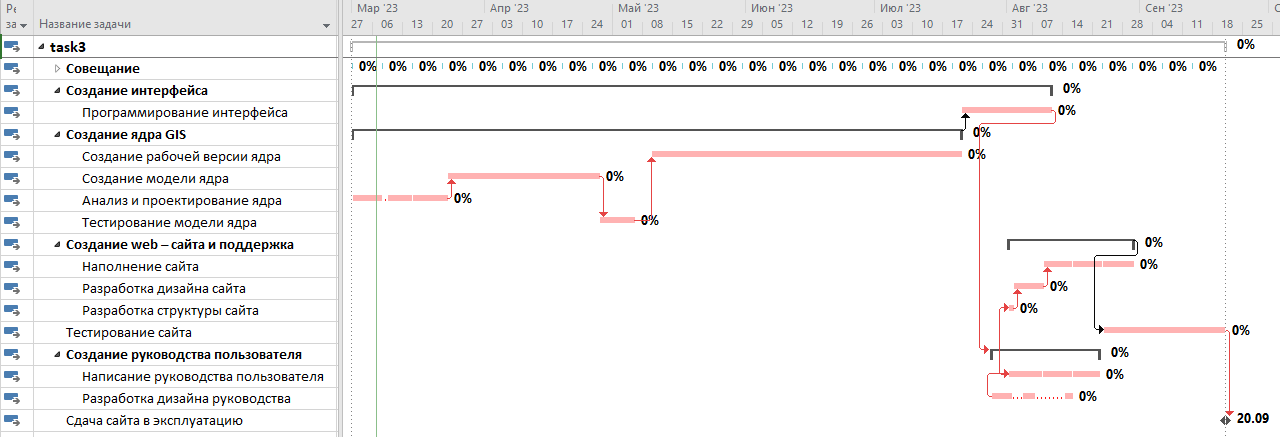
\includegraphics[width=1\linewidth]{inc/img/7.png}
	\caption{Критический путь}
	\label{p7}
\end{figure}

Для уменьшения срока реализации проекта были назначенны дополнительные ресурсы на задачи использующие программистов (рис. \ref{p8}).

\newpage
\begin{figure}[!h]
	\centering
	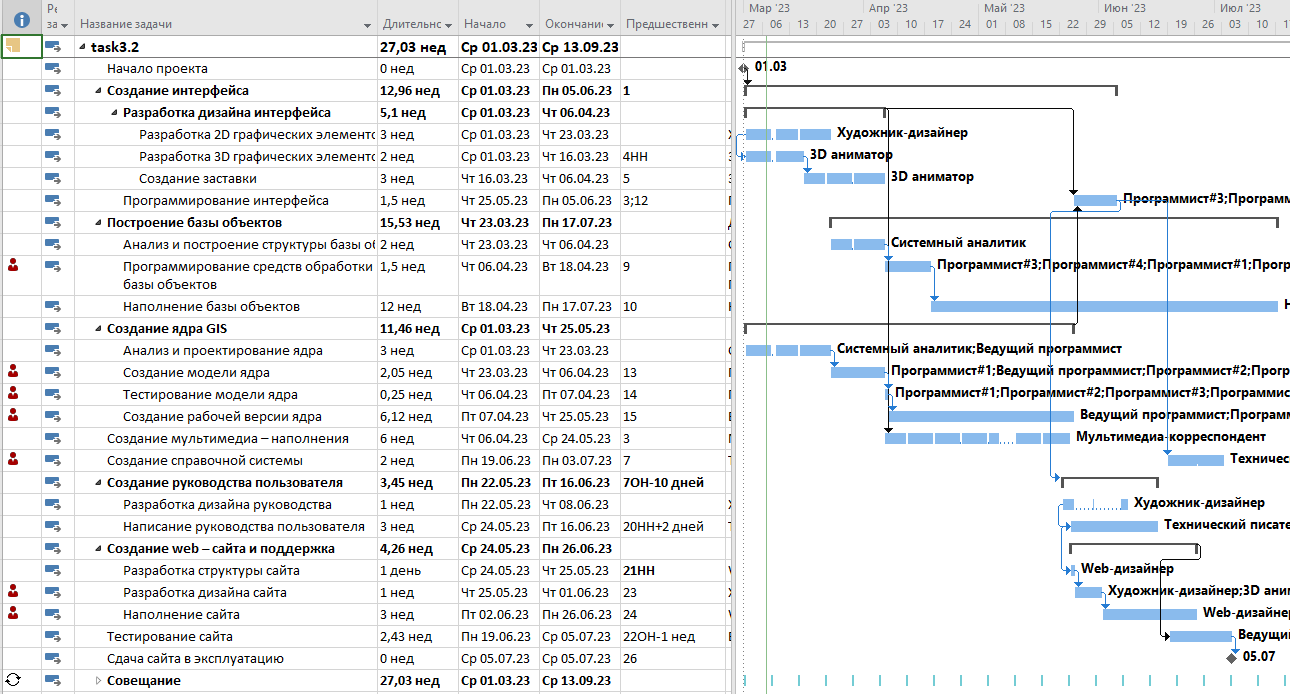
\includegraphics[width=1\linewidth]{inc/img/8.png}
	\caption{Дополнительное назначение ресурсов}
	\label{p8}
\end{figure}

На рисунке \ref{p9} можно увидеть диаграмму Ганта после ликвидации перегрузки ресурсов.

\begin{figure}[!h]
	\centering
	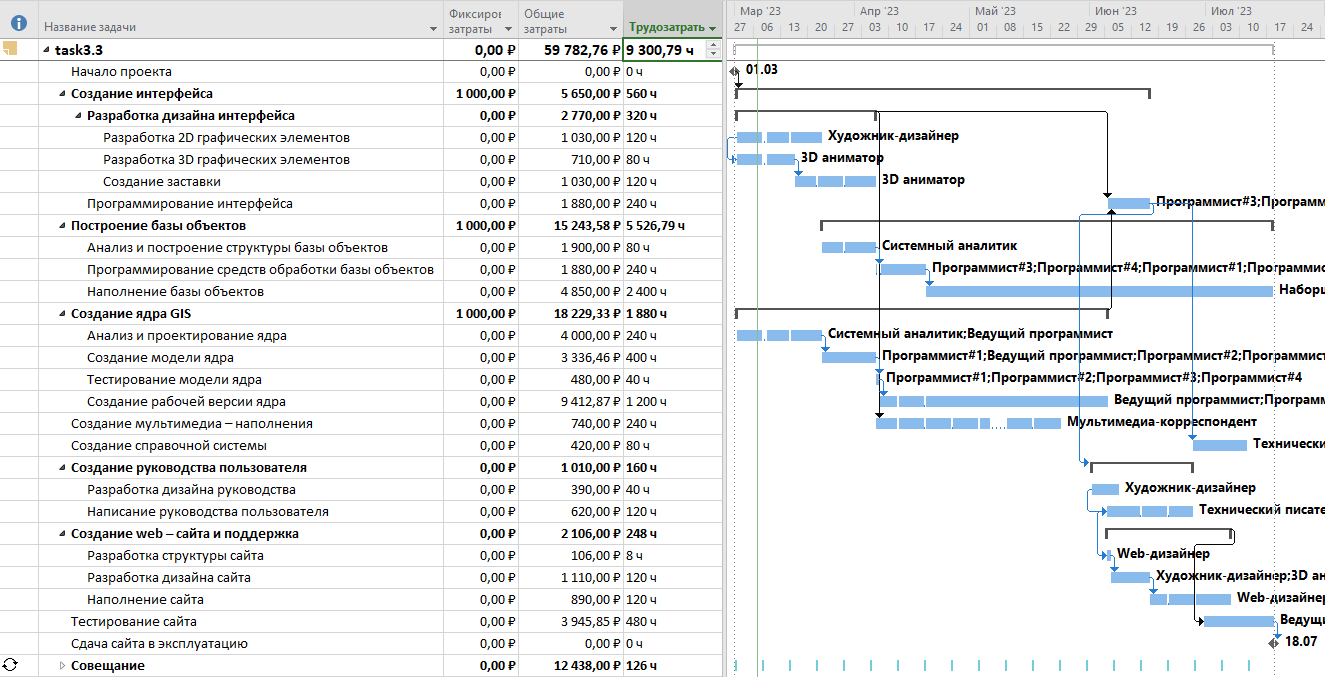
\includegraphics[width=1\linewidth]{inc/img/9.png}
	\caption{Диаграмма Ганта после устранения перегрузки}
	\label{p9}
\end{figure}

\newpage
На рисунке \ref{d1} изображена диаграмма затрат по группам ресурсов.
\begin{figure}[!h]
	\centering
	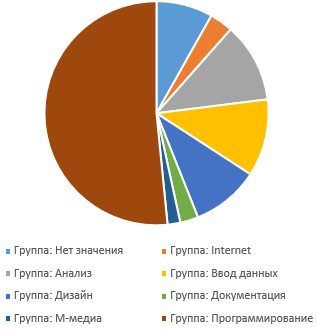
\includegraphics[width=0.6\linewidth]{inc/img/d1.png}
	\caption{Диаграмма затрат по группам ресурсов}
	\label{d1}
\end{figure}

На рисунке \ref{d2} изображена диаграмма трудозатрат по тем же группам ресурсов.
\begin{figure}[!h]
	\centering
	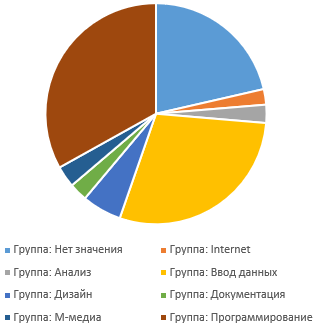
\includegraphics[width=0.6\linewidth]{inc/img/d2.png}
	\caption{Диаграмма трудозатрат по группам ресурсов}
	\label{d2}
\end{figure}

\section*{Выводы}
По сравнению с диаграммами из ЛР №2, из-за добавления совещаний, затраты на анализ увеличились больше чем в 2 раза (10 360,00 руб.), на дизайн почти в 2 раза (6 748,00 руб.), а затраты на программистов выросли незначительно. Из этого можно сделать вывод что зарплаты аналитиков и дизайнеров выше чем у остальных. При этом соотношение трудозатрат по группам почти не изменилось.

По итогу проделанной работы были получены навыки оптимизации параметров проекта, выравнивания загрузки ресурсов и учета периодических задач, а также получилось минимизировать критический путь.